\startchapter{Density Experiment}
\label{chapter:newsol}

\subsection{Introduction}

 The \textit{Density Experiment} was conducted in the summer of 2015 \citep{fishforensics,hatchery}. The goal was to investigate the relationship between Transformed CT values (`TCT') and Coho Salmon `density’ (or the similar measurement of biomass). CT is the `Cycle Threshold' and we define TCT=50-CT.  The experiment consisted of manipulating juvenile Coho salmon densities in treatments of 1, 2, 4, 8, 16, 32, and 65 fish in replicated 10,000L tanks.


\begin{figure}[H]
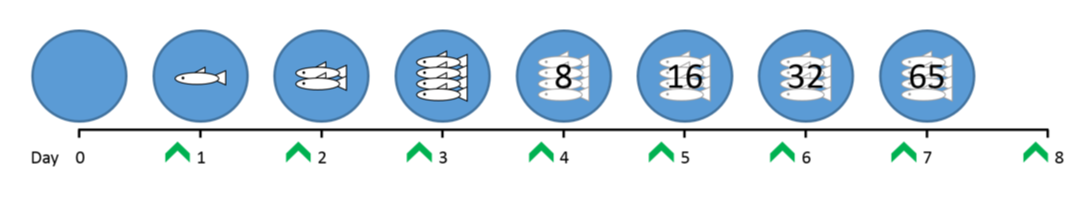
\includegraphics[scale=0.6]{Chapter3Images/samplingscheduleday.png}
\caption{ Sampling schedule for the Density Experiment \citep{berg}.}
\label{fig:densityschedule1}
\end{figure}

Figure~\ref{fig:densityschedule1}  \citep{fishforensics} provides an overview of the experimental schedule. For each main tank, Coho were added throughout the week of the experiment (indicated by the green arrows). On day one, one fish was added to the tank. On each of the following days of the week, fish were added until on day 7 there were 65 fish.

\vspace{3mm}

There were four 10,000L Tanks, numbered 19, 20, 21 and 24 for the main density experiment. From each tank, sample replicates of water were taken, usually five per tank.
For each fish, the biomass in grams was also recorded. The average mass of each fish used in the experiment was 5.69 grams. As the amount of water in each tank in this experiment was fixed, we expect that as biomass increases, the CT score should decrease (as we would expect more eDNA);  hence, the TCT should increase.

\begin{figure}[H]
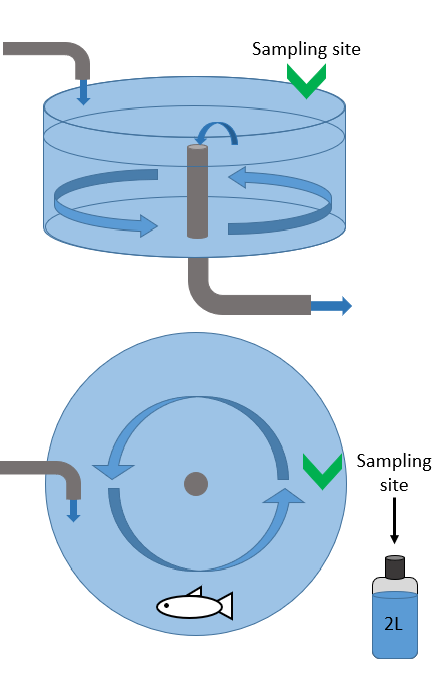
\includegraphics{Chapter3Images/goldstreamupdate.png}
\caption{The general sampling methodology for the density experiment \citep{berg}.}
\label{fig:samplingdensity}
\end{figure}

\newpage

Figure~\ref{fig:samplingdensity} illustrates the method in which samples were taken from the tanks. To sample from the tanks, 2L bottles were filled with water by submersion approximately 0.5m from the edge of the tank. The water was then filtered through 47mm diameter 0.45$\mu$m mixed-cellulose ester (MCE) filter membranes. From each sample replicate, eight technical replicates were obtained. These technical replicate samples were then evaluated using qPCR for the presence of Coho eDNA. Each unique set of eight technical replicates were assigned a unique ``sort.code". That is, every member that came from the same group of eight technical replicates had the same sort code. Note that one set of technical replicates, corresponding to sort.code=128 was discarded before analysis due to lack of integrity in the lab (Sample.replicate 3 of Tank 20, 65 Fish). 

\vspace{5mm}

In order to detect Coho salmon specifically, a DNA assay,  eONKI4 was used in combination with qPCR. To ensure quality of the eDNA, samples first underwent integritE-DNA tests. These tests combine a probe and a primer to amplify chloroplast DNA that appear pervasively in freshwater systems. Samples that failed the integritE-DNA test were cleaned using the Zymo OneStepTM PCR Inhibitor Removal Kit  and tested again. If the sample failed a second time, it underwent an inhibitor removal. If the sample still failed to pass the integritE-DNA test after inhibitor removal, it was excluded from the data to minimize the presence of false negatives. The qPCR analysis using the eONKI4 assay was conducted in the lab of Dr. Caren Helbing at the University of Victoria. Figure~\ref{fig:densityschedule} is a visualization of the process of DNA integrity validation. integritE-DNA tests were performed on samples prior to using qPCR to search for Coho eDNA. Before the experiment began, the tanks were bleached to clean any residual eDNA or materials that may have been present in the tanks. integritE-DNA test combines a probe and a primer to amplify chloroplast DNA that is pervasive in freshwater systems. 

\vspace{5mm}


For 1, 2, 4, 8, 16, and 32 fish, 6*4*5*8=960 observations were recorded. For each set of these six numbers of Coho, there were four tanks, for each tank there were five sample replicates, and for each sample replicate there were eight technical replicates.
For 65 Fish, there were 3*5*8+4*8=152 observations. For 65 fish there were three tanks with five sample replicates and one tank with four, for each sample replicate there were eight technical replicates.

\vspace{5mm}

A small pilot experiment was also conducted during the summer. The pilot experiment used smaller tanks, tanks 1, 2, 3 and 4.  Samples were taken from smaller tanks that only contained hatchery water and no Coho. The pilot experiment was used to gain insight regarding possible background signals in the hatchery waters.



\begin{figure}[H]
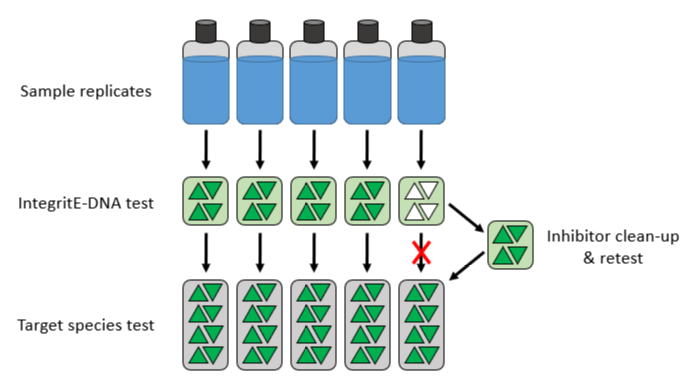
\includegraphics[scale=0.75]{Chapter3Images/integritE.png}
\caption{ Basic procedure for analyzing eDNA. Sample replicates were first certified using an integritE-DNA test before testing for Coho eDNA \citep{berg}.}
\label{fig:densityschedule}
\end{figure}

